\documentclass[tikz,border=6pt]{standalone}
\usepackage{pgfplots}
\pgfplotsset{compat=1.18}
\usepgfplotslibrary{colormaps}
\usetikzlibrary{arrows, arrows.meta, calc}
\usetikzlibrary{decorations.markings}


\usepackage{amssymb,amsmath,mathtools}

\usepackage[T1]{fontenc}
\usepackage[utf8]{inputenc}
\usepackage{newpxtext,newpxmath}
\usepackage{sectsty}

\renewcommand{\Re}{\operatorname{\mathrm{Re}}}
\renewcommand{\Im}{\operatorname{\mathrm{Im}}}

\begin{document}
	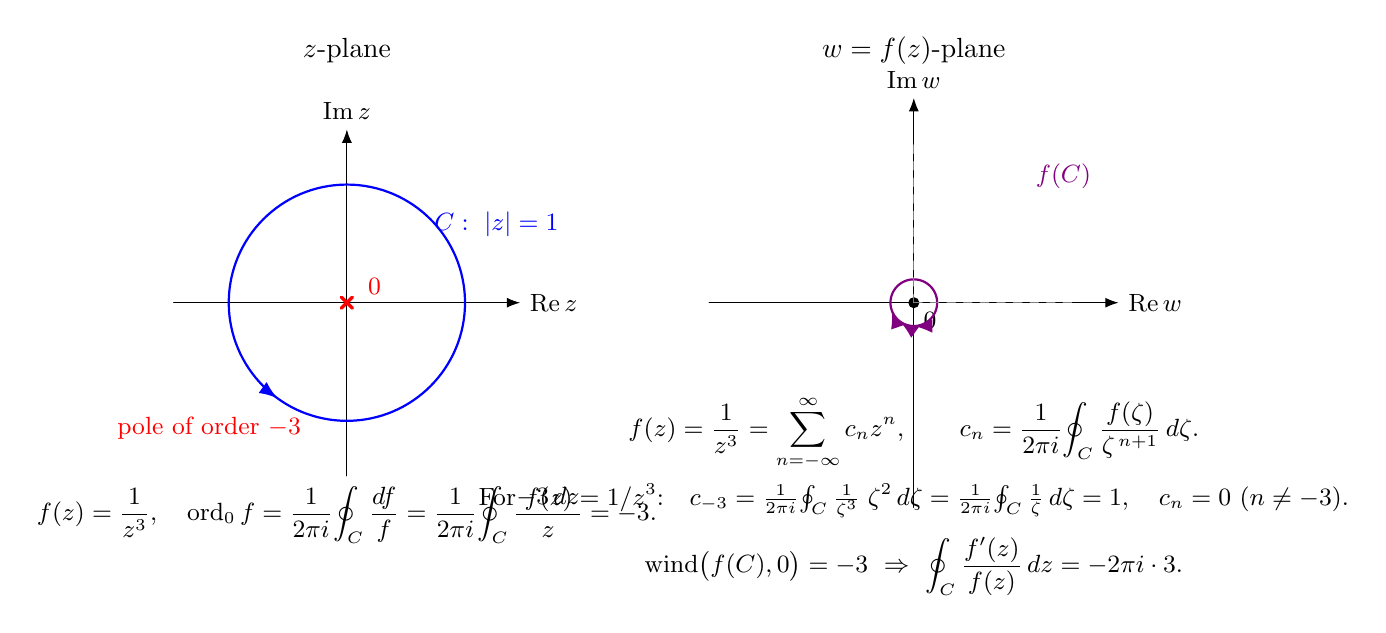
\begin{tikzpicture}[>=Latex, line cap=round, line join=round, font=\small]
		
		%========================
		% Left: z-plane
		%========================
		\begin{scope}[shift={(0,0)}]
			\node[font=\normalsize] at (0,3.2) {$z$-plane};
			% axes
			\draw[->] (-2.2,0)--(2.2,0) node[right] {$\Re z$};
			\draw[->] (0,-2.2)--(0,2.2) node[above] {$\Im z$};
			
			% unit circle C (positively oriented) -- radius 1.5 for visibility
			\draw[blue,thick,postaction={decorate},
			decoration={markings, mark=at position 0.65 with {\arrow{>}}}]
			(0,0) circle (1.5);
			\node[blue] at (1.9,1.0) {$C:\ |z|=1$};
			
			% pole at 0 (order -3)
			\draw[red,very thick] (0,0) ++(-0.07,-0.07) -- ++(0.14,0.14);
			\draw[red,very thick] (0,0) ++(-0.07,0.07)  -- ++(0.14,-0.14);
			\node[red] at (0.35,0.2) {$0$};
			\node[red] at (-1.75,-1.6) {pole of order $-3$};
			
			% function label + order via winding/logarithmic derivative
			\node[align=left] at (0,-2.7) {$\displaystyle
				f(z)=\frac{1}{z^{3}},\quad
				\operatorname{ord}_{0} f
				=\frac{1}{2\pi i}\!\oint_C \frac{df}{f}
				=\frac{1}{2\pi i}\!\oint_C \frac{-3\,dz}{\,z\,}=-3.$};
		\end{scope}
		
		%========================
		% Right: w-plane = f(z)-plane
		%========================
		\begin{scope}[shift={(7.2,0)}]
			\node[font=\normalsize] at (0,3.2) {$w=f(z)$-plane};
			% axes
			\draw[->] (-2.6,0)--(2.6,0) node[right] {$\Re w$};
			\draw[->] (0,-2.6)--(0,2.6) node[above] {$\Im w$};
			
			% origin
			\fill (0,0) circle(2pt) node[below right] {$0$};
			
			% image curve f(C): z = 1.5 e^{it} -> w = (1/1.5^3) e^{-i 3t}
			\draw[violet,thick,
			postaction={decorate},
			decoration={markings,
				mark=at position 0.15 with {\arrow{>}},
				mark=at position 0.45 with {\arrow{>}},
				mark=at position 0.75 with {\arrow{>}}}]
			plot[domain=0:6.283, samples=600]
			({ (1/(1.5*1.5*1.5))*cos(3*\x r) },
			{ -(1/(1.5*1.5*1.5))*sin(3*\x r) }); % clockwise triple winding
			\node[violet] at (1.9,1.6) {$f(C)$};
			
			% dashed rays to visualize winding
			\draw[gray,dashed] (0,0) -- (2.1,0);
			\draw[gray,dashed] (0,0) -- (0,2.1);
			
			% annotation: Laurent coefficients via Cauchy integrals (about 0)
			\node[align=center] at (0,-2.45)
			{$\displaystyle
				f(z)=\frac{1}{z^{3}}=\sum_{n=-\infty}^{\infty} c_n z^n,\qquad
				c_n=\frac{1}{2\pi i}\!\oint_C \frac{f(\zeta)}{\zeta^{\,n+1}}\,d\zeta.$\\[4pt]
				For $f(z)=1/z^{3}$:\quad
				$c_{-3}=\frac{1}{2\pi i}\!\oint_C \frac{1}{\zeta^{3}}\;\zeta^{2}\,d\zeta
				=\frac{1}{2\pi i}\!\oint_C \frac{1}{\zeta}\,d\zeta=1,\quad
				c_n=0\ (n\neq -3).$\\[6pt]
				$\mathrm{wind}\big(f(C),0\big)=-3
				\ \Rightarrow\
				\displaystyle \oint_C \frac{f'(z)}{f(z)}\,dz=-2\pi i\cdot 3.$};
		\end{scope}
		
	\end{tikzpicture}
\end{document}